\section{Consultar Doctor}

Un paciente contará con la facultad de consultar los doctores que son o fueron
responsables de sus tratamientos y así poder tener un conocimiento de éstos.

\subsubsection{Procedimiento}
\begin{enumerate}
	
	\item Da clic en el icono \textbf{Doctores} de la pantalla \textbf{Menú Principal}.

		\begin{figure}[!htbp]			\hypertarget{fig:mpPaciente8}{\hspace{1pt}}
		\begin{center}
			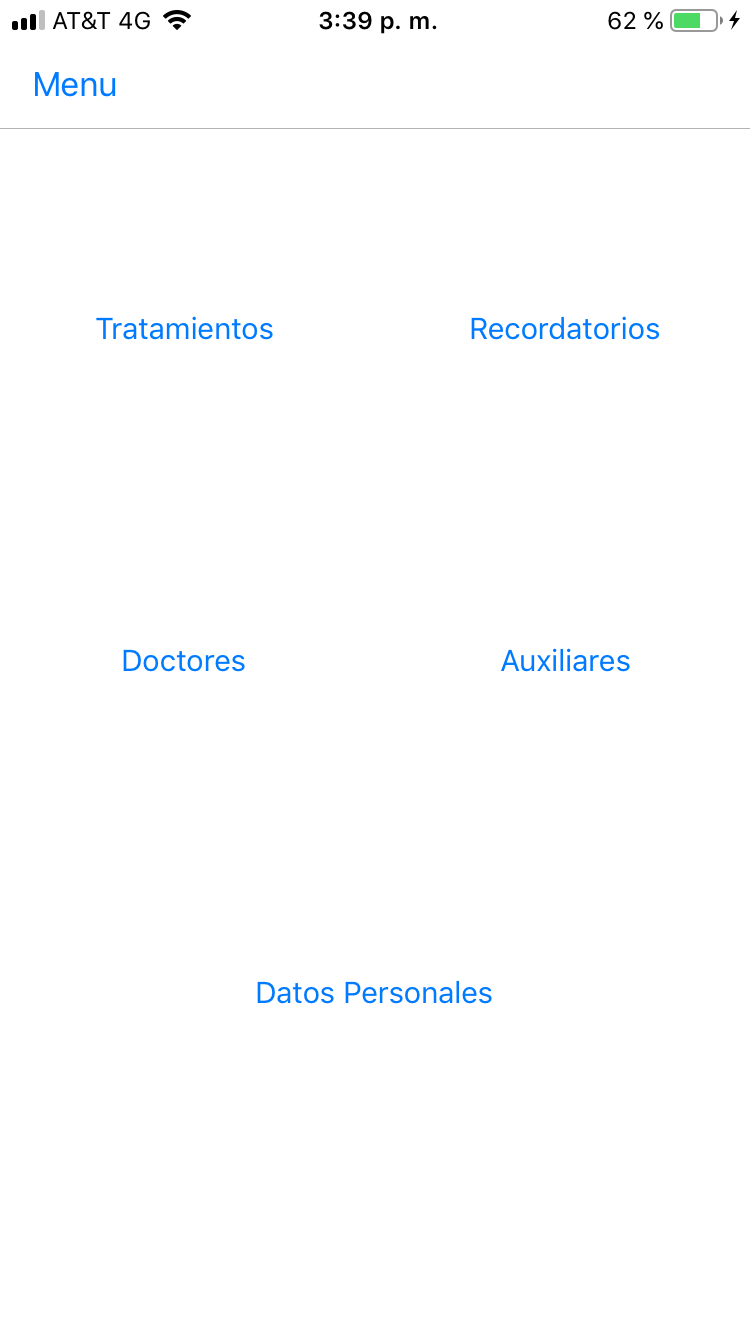
\includegraphics[height=0.4\textheight]{Paciente/ConsultarDoctor/images/mpPaciente}
			\caption{Menú Principal Paciente}
			\label{fig:mpPaciente8}
		\end{center}
	\end{figure}

	\item Se mostrará la pantalla \textbf{Doctores}. 
	\newpage
	\begin{figure}[!htbp]			
		\hypertarget{fig:Doctores}{\hspace{1pt}}
		\begin{center}
			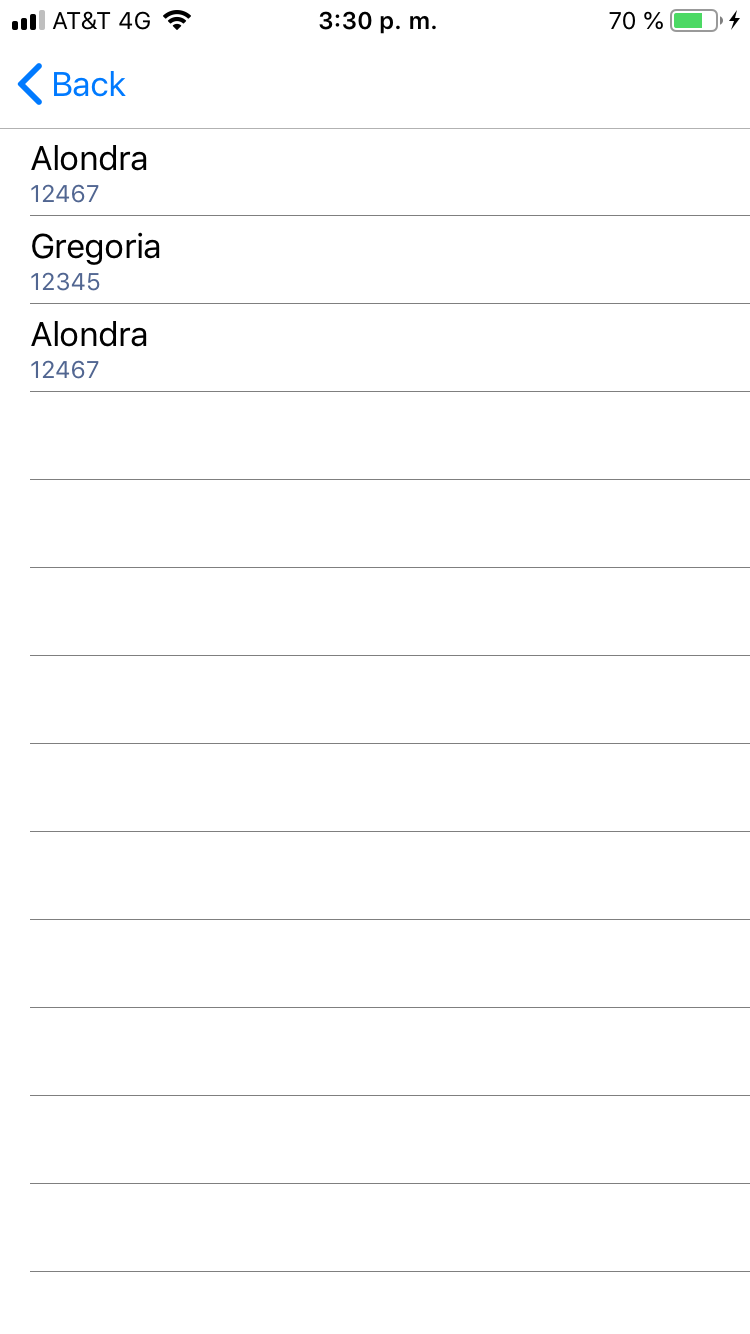
\includegraphics[height=0.4\textheight]{Paciente/ConsultarDoctor/images/Doctores}
			\caption{Doctores}
			\label{fig:Doctores}
		\end{center}
	\end{figure}

	
\end{enumerate}

